\section{Changing the equation of state}
Following~\cite{Ma1995}, the background energy and pressure for massive neutrinos are given by
\begin{equation}\label{eq:dens-press-massive-nu}
    \rho_\nu = a^{-4} \int q^2\,  \ddif q\, \ddif\Omega\,  \varepsilon\,  f_0(q)\, ,\qquad
    P_\nu = \frac{1}{3}a^{-4} \int q^2\, \ddif q\,  \ddif\Omega\, \frac{q^2}{\varepsilon}\, f_0(q) \, ,
\end{equation}with $\varepsilon = \sqrt{q^2 + m_\nu^2 a^2}$. In the ultra-relativistic limit $\varepsilon\sim q$, $P_\nu = \frac{1}{3}\rho_\nu$, i.e. $w = 1/3$. Also, both $\rho$ and $p$ evolve as $a^{-4}$. In the non-relativistic limit, $a^2m_\nu^2\gg q^2$, and then $P_\nu \to 0$, such that $w = 0$. Now, $\rho$ evolves with $a^{-3}$ due to the $a$ factor in $\varepsilon$. The mass naturally introduces a phase transition between $w = 1/3$ and $w=0$, and the $\rho$ evolution varies smoothly from $a^{-4}$ to $a^{-3}$. 

Massless neutrinos with $m_\nu=0$ fulfill $\varepsilon = q$ and then \eqref{eq:dens-press-massive-nu} becomes 
\begin{equation}\label{eq:dens-press-massless-nu}
    \rho_\nu = a^{-4}  \int q^2\,  \ddif q \, \ddif \Omega\,  q\,  f_0(q)\, ,\qquad
    P_\nu = \frac{1}{3}\, a^{-4} \int q^2\, \ddif q\,  \ddif \Omega\,  q\,  f_0(q) \, .
\end{equation}That is, massless neutrinos always have $w = 1/3$. 

\subsection{Arbitrary equation of state}
From the energy-momentum tensor conservation, we can retrieve
\begin{equation}
    \frac{\ddif \rho}{\rho} = -3\, \frac{\ddif a}{a}\, (1+w(a))\, 
\end{equation}for an arbitrary equation of state $w(a)$. The solution is trivial,
\begin{equation}\label{eq:rho-solution}
    \rho(a) = \rho_{\mathrm{ini}} \exp\left\{-3\int_{a_{\mathrm{ini}}}^a \frac{da'}{a'}(1+w(a')) \right\}\, .
\end{equation}
Then, we modify the massless neutrino energy density and pressure as follows:
\begin{align}\label{eq:eos-energy-density}
    \rho_\nu &= a_{\mathrm{ini}}^{-4}\, \exp\left\{-3\int_{a_{\mathrm{ini}}}^a \frac{da'}{a'}(1+w(a')) \right\}\int q^2\,  \ddif q \, \ddif \Omega\,  q\,  f_0(q)\, ,\qquad \\
    P_\nu &= a_{\mathrm{ini}}^{-4}\, w(a)\exp\left\{-3\int_{a_{\mathrm{ini}}}^a \frac{da'}{a'}(1+w(a')) \right\} \int q^2\, \ddif q\,  \ddif \Omega\,  q\,  f_0(q) \, . \label{eq:eos-pressure}
\end{align}This way, we necessarily have $P_\nu/\rho_\nu = w(a)$ and the correct evolution with $a$ during all history. 
One can understand this formula as setting~\eqref{eq:dens-pres-massless-nu} inside~\eqref{eq:rho-solution}.

\subsection{Different parametrisations for $w(a)$}
A first possibility is to try to fit if neutrinos go non-relativistic. We introduce an equation of state which goes from UR to NR in a single step at $a = a_{\text{tr}}$,
\begin{equation}\label{eq:one-step-eos}
    w(a) = \begin{cases}
        1/3 & a < a_{\text{tr}}\\ 0 & a > a_{\text{tr}}
    \end{cases}\, .
\end{equation}We expect cosmology to put a bound on $a_{\text{tr}}$ in the same manner that it can put a bound on $m_\nu$. 

However, we can do an arbitrary number of steps $n$,
\begin{equation}
    w(a) = \begin{cases}
        1/3 & a < a_{0}\\ w_{i} & a_{i-1} < a < a_{i} \\ w_{n} & a > a_{n-1}
    \end{cases}\, ,
\end{equation}with $i = 1, \ldots, n$.

\section{CLASS results}
In the following examples, we fix $\omega_b, \omega_{\mathrm{cdm}}, \theta_s, A_s, n_s, \tau_{\mathrm{reio}}$ to their $\Lambda$CDM values, and vary the amount of neutrinos and their equation of state. 

We want to compare a single massive neutrino with $m_\nu = 0.33\, \mathrm{eV}$ to a signle massless neutrino with an equation of state which tries to mimic the mass. The three different equations of state for this neutrino are shown in figure~\ref{fig:equation-of-states}. The other two neutrinos are massless with $w = 1/3$. 
\begin{figure}
    \centering
    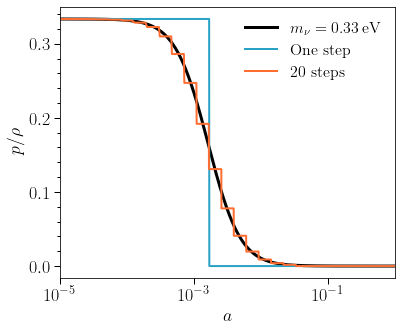
\includegraphics[width = 0.7\textwidth]{"Figures/eos_330meV.png"}
    \caption{Evolution of the equation of state with the scale factor. In black, the equation of state corresponding to a $m_\nu = 0.33\, \mathrm{eV}$. In blue, a single-step equation of state which transitions at $a_{\mathrm{tr}} = 1.5\times 10^{-3}$. In orange, a 20-step equation of state which mimics the behaviour of its mass analogous.}
    \label{fig:equation-of-states}
\end{figure}

First of all, in figure~\ref{fig:energy-and-pressure} we can see that the energy density and pressure of this neutrino species both evolve as expected. The energy density and pressure defined in (\ref{eq:eos-energy-density}) and (\ref{eq:eos-pressure}) correctly match the mass evolution. 

\begin{figure}
    \centering
    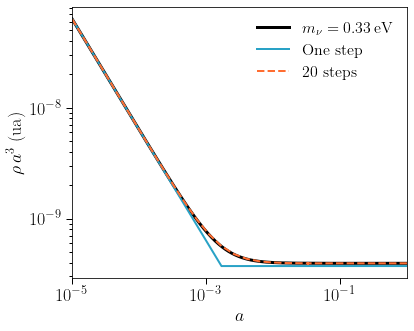
\includegraphics[width = 0.495\textwidth]{"Figures/energy_density_330meV.png"}
    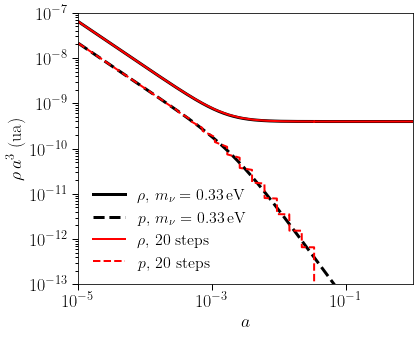
\includegraphics[width = 0.495\textwidth]{"Figures/pressure_330meV.png"}
    \caption{Evolution of the energy density and pressure. In black, a massive neutrino with $m_\nu = 0.33\, \mathrm{eV}$. In blue and orange (and red), a massless neutrino with the equation of state from figure~\ref{fig:equation-of-states}.}
    \label{fig:energy-and-pressure}
\end{figure}

We expect the background contribution from three cases to be, at least, similar. As shown in figure~\ref{fig:cmb-bad-perturbations}, we compute the CMB anisotropies and find that, well, they are not. Adding additional steps to the equation of state helps to reproduce the oscillations at large multipoles, but the matching is far from good, specially at small multipoles. Note, however, that the perturbations have not been modified and, in the three cases, they are the ones from massive neutrinos.
\begin{figure}
    \centering
    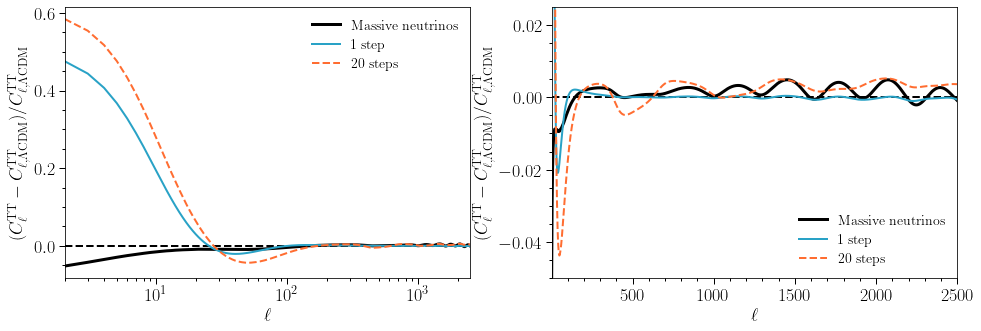
\includegraphics[width = \textwidth]{"Figures/cmb_330meV_badpert.png"}
    \caption{Difference of CMB anisotropies with respect to the $\Lambda$CDM model with three massless neutrinos. NCDM perturbations are on as if the neutrino were massive. Left, multipoles in log scale. Right, multipoles in linear scale. In black, a massive neutrino with $m_\nu = 0.33\, \mathrm{eV}$. In blue and orange, a massless neutrino with the equation of state from figure~\ref{fig:equation-of-states}.}
    \label{fig:cmb-bad-perturbations}
\end{figure}


Then, what happens if we turn off the contribution of the ``massive'' neutrino (or that with an arbitrary equation of state) to perturbations? Well, in figure~\ref{fig:cmb-no-perturbations} we can see that the matching to the CMB anisotropies is almost exact, specially for the 20-step equation of state case. 
\begin{figure}
    \centering
    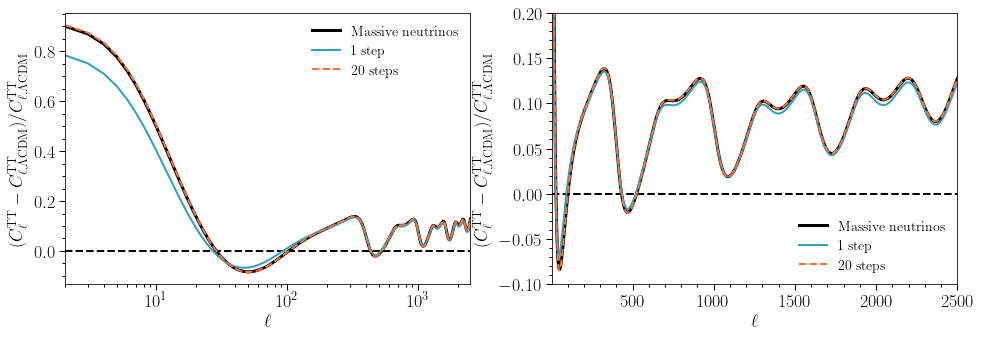
\includegraphics[width = \textwidth]{"Figures/cmb_330meV_nopert.png"}
    \caption{Difference of CMB anisotropies with respect to the $\Lambda$CDM model with three massless neutrinos. NCDM perturbations are off. Left, multipoles in log scale. Right, multipoles in linear scale. In black, a massive neutrino with $m_\nu = 0.33\, \mathrm{eV}$. In blue and orange, a massless neutrino with the equation of state from figure~\ref{fig:equation-of-states}.}
    \label{fig:cmb-no-perturbations}
\end{figure}

If this is true, it would mean that perturbations are important and not negligible with respect to the background. There is something in the effect of neutrinos that is not directly reproduced by the equation of state on the background. We must now discover what.

\section{A fit to the mass of the neutrino}
Now we repeat the same exercise and try to see which bound does the Planck data put on our models. We compare one massive neutrino, with one massless neutrino described by a one-step equation of state like~(\ref{eq:one-step-eos}). The free parameters are $m_\nu$ and $a_{\mathrm{tr}}$, respectively. The prior distribution is flat in $\log a_{\mathrm{tr}}\in (-4.2,0)$. The posterior distributions from a relatively-short chain are shown in figure~\ref{fig:posteriors}. By absolutely rough ocular inspection, we see that the data prefers $a_{\mathrm{tr}}\gtrsim 10^{-2.5}\sim 3\times 10^{-3}$, which roughly corresponds to a mass bound $m_\nu \lesssim 0.17\, \mathrm{eV}$. Contrarily, the fit to $m_\nu$ gives $m_\nu \lesssim 0.1\, \mathrm{eV}$, which is twice as constringent. Maybe the $\log a_{\mathrm{tr}}$ does not fall as steeply as it should, but the order of magnitude is, at least, correct.
\begin{figure}
    \centering
    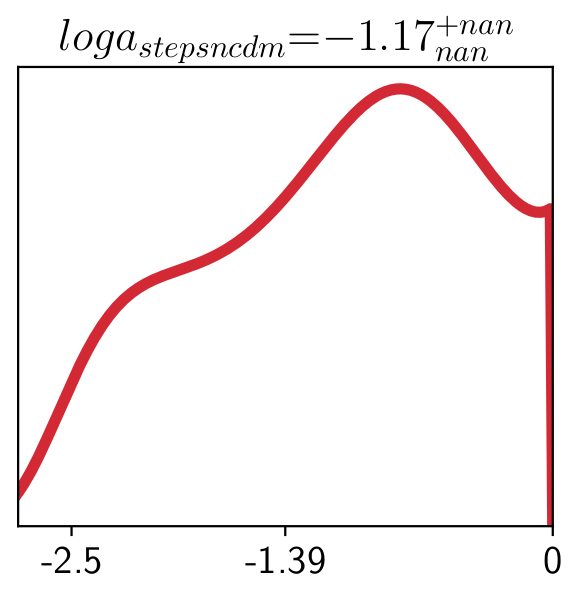
\includegraphics[width = 0.495\textwidth]{"Figures/posterior-onestep.png"}
    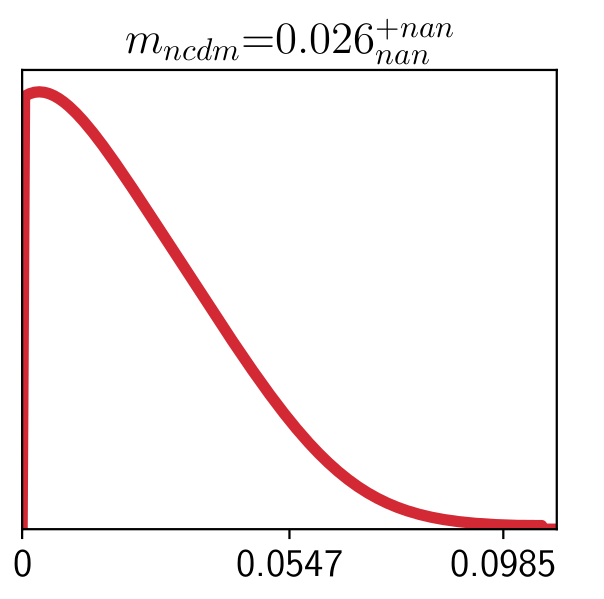
\includegraphics[width = 0.495\textwidth]{"Figures/posterior-mass.png"}
    \caption{Posterior distributions for $\log a_{\mathrm{tr}}$ and $m_\nu$.}
    \label{fig:posteriors}
\end{figure}

If it's of any interest, I attach in figure~\ref{fig:mcmc-points} the values of $m_\nu$ and $a_{\mathrm{tr}}$ in the MontePython MCMC. As one can see, the MCMC avoids sampling points with small scale factor or large mass.
\begin{figure}
    \centering
    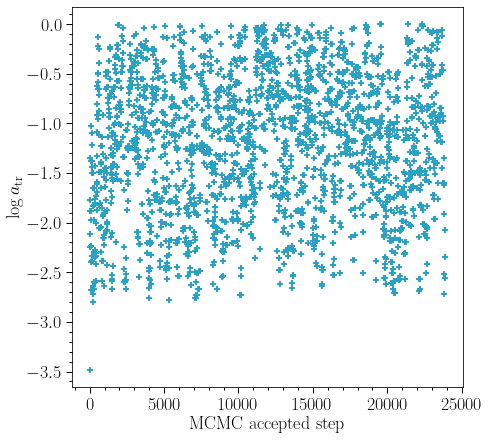
\includegraphics[width = 0.495\textwidth]{"Figures/mcmc-onestep.png"}
    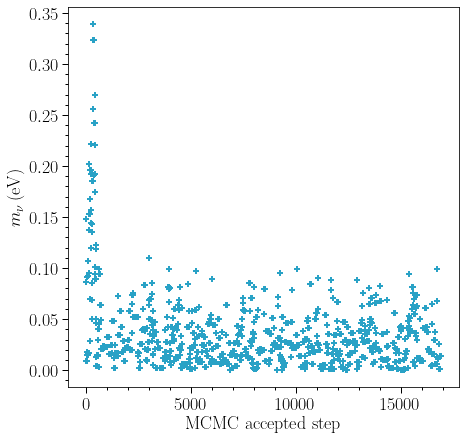
\includegraphics[width = 0.495\textwidth]{"Figures/mcmc-mass.png"}
    \caption{Sampled points during the MCMC for $\log a_{\mathrm{tr}}$ and $m_\nu$.}
    \label{fig:mcmc-points}
\end{figure}
